\newpage

\section{Bandwidth}
In \opnsense, bandwidth limitation is called shaper and can be found in the menu \cmd{Firewall --> Shaper}. There are many reasons for implementing a bandwidth limitation solution. It could be to prioritize certain network traffic or optimize the bandwidth that is used. Some other vendors could call this for \textbf{QoS}, Quality of Service.

In this section, you will learn:
\begin{itemize}
    \item Create a bandwidth limitation rule.
    \item The difference between using a pipe and a queue.
\end{itemize}

To create a bandwidth limitation, you first need to create a pipe and then assign that pipe to an interface using the rule configuration. The first step is to create a pipe:

\setupblock{\begin{enumerate}
    \item Goto \cmd{Firewall --> Shaper --> Pipe}. A pipe defines the speed you set.
    \item Change \cmd{Bandwidth} to the amount you want. For this to work in this tutorial, it needs to be lower than the speed you get from your ISP. For example, 10.
    \item Change \cmd{Bandwidth Metric} to the correct designation. For example, \cmd{Mbit/s}. % is designation the correct word to use?
    \item And give it a \cmd{Description} that describes what this pape does. For example, ''10mbps''.
    \item Click on \cmd{Save} and \cmd{Apply}.
\end{enumerate}}

Now, you have created a pipe that can be used in a rule to limit bandwidth. The next step is to create the rule:

\setupblock{\begin{enumerate}
    \item Goto \cmd{Firewall --> Shaper --> Rule}. This defines where the pipe should apply.
    \item Set the \cmd{Sequence} to \cmd{1}.
    \item Set \cmd{Interface} to WAN.
    \item Set \cmd{Proto} to \cmd{ip}.
    \item Set \cmd{Source} and \cmd{Destination} to \cmd{All}.
    \item And set \cmd{Target} to the pipe you created earlier (10mbps).
    \item Click on \cmd{Save} and \cmd{apply} to create and start the rule.
\end{enumerate}}

\quesblock{\begin{enumerate}
    \item[29.] Test the configuration you have made using a site that can do a speed test. Do you get the same result as in figure \ref{opnsense:bandwidth_speed}?
    \item[30.] How can you use this rule against on IP instead of all on the interface? 
    \item[31.] There is also one more configuration that can be done, \cmd{queues}. What does it do?
    \item[32.] Why would you prioritize some traffic over other traffic?
\end{enumerate}}

\begin{figure}[h!]
    \centering
    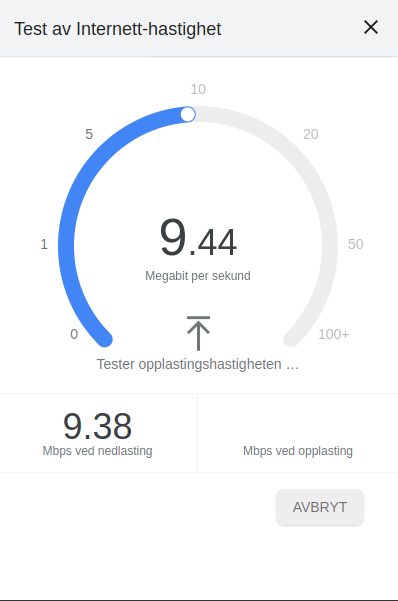
\includegraphics[width=0.3\textwidth]{Images/bandwidth/up_down.PNG}
    \caption{Google speedtest}
    \label{opnsense:bandwidth_speed}
\end{figure}

\subsection{Queue}
Using the \cmd{Queue} options implement the WF2Q+ (Worst-case Fair Weighted Fair Queueing) policy. The queue is associating a \textbf{weight} and a pipe to a flow. The difference between a pipe and a queue is that a pipe is a hard limit, while a queue is used to share the bandwidth in a pipe, based on the ''weight'' that is used. There can be multiple queues in a pipe.

The configuration of a queue is almost the same as when you created a pipe. The only difference is that you need to choose a pipe the queue is going to use and the weight (1 - 100) the queue has (see figure \ref{opnsense:bandwidth_queue}). The lower weight, the more prioritized it is.

\begin{figure}[h!]
    \centering
    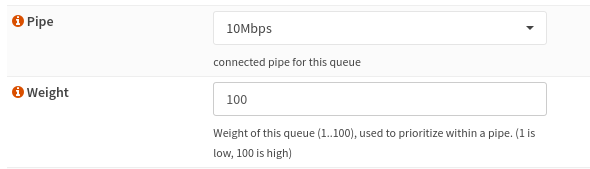
\includegraphics[width=0.6\textwidth]{Images/bandwidth/queue.PNG}
    \caption{Queue configuration differences from pipe configuration}
    \label{opnsense:bandwidth_queue}
\end{figure}

\quesblock{\begin{enumerate}
    \item[33.] How can you test if the queue is working?
\end{enumerate}}

\subsection{Status}
The \cmd{Status} will show you which bandwidth limitation that is implemented on the firewall at all time. Only rules, pipes, and queues that are \cmd{Enabled} will be shown on the status page. An example with the rule created in the first task in this section can be seen in \ref{opnsense:bandwidth_status}.

\begin{figure}[h!]
    \centering
    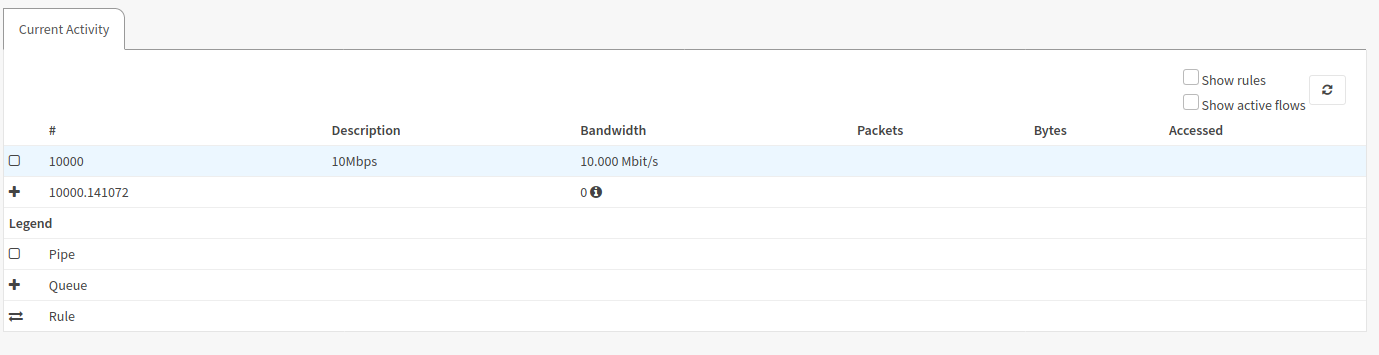
\includegraphics[width=0.8\textwidth]{Images/bandwidth/status.PNG}
    \caption{Shaper status}
    \label{opnsense:bandwidth_status}
\end{figure}

\tipbox{Only pipes, queues, and rules that are \cmd{enabled} will be displayed on the status page.}
